\chapter{Morse functions on point clouds}

In this chapter we introduce a quite succesful technique introduced by: 
F. Cazals, A.Roth, C. Robert, M. Christian
in \cite{caz2013}.

This technique focuses on discrete augmented metric spaces.
In particular, suppose we have a compact smooth manifold
$M$ equipped with a Morse function $f:M\to \mathbb{R}$.

Usually this Morse function $f$ will be the height function.

From this manifold $M$ we sample a finite amount of points 
$X=\{x_i\}_{i=0}^n$ and we record the value of $f$ on $X$.

As usual, we investigate what sort of topological information we can recover from this
discrete sample.


The basic idea is the following: Suppose we are in dimension $n$,
then we iterate $n$ times. On each iteration we build a graph around with vertices in $X$.
Our hope is that as we build this graph it will be natural to identify the critical points of $f$ as
well as their indices.

\section{Pseudo-gradient graphs}

The first thing we would like to do is recover the gradient of the function $f$.
For this purpose we create a graph using $X$ as its base set
and we define a flow on the graph by moving from one point to the point
connected with it where the morse function $f$ takes the smallest value.

\begin{definition}[NNG graph]

Given $X$ a discrete set,
we define $G^-(X)$ it's descending pseudo-gradient graph
as the nearest neighbour graph of $X$. 

That is the graph where the 
edges $\{x_i,x_j\}$ are precisely where either $d(x_i,x_j)=d(x_i,X)$
or $d(x_i,x_j)=d(x_j,X)$. 

Notice that the binary relation $x_i\sim x_j$ if 
and only if
$x_j$ is the closest vertex to $x_i$ is not symmetric.

We denote as $\omega^-:G\to G$ the application that
maps $p\in X$ to the result of iteratively following the point
with that its joined to $p$ and that minimises the value of $f$.

We define $\alpha^-$ in an analogous manner, by following the direction 
of maximum growth of $f$.
\end{definition}

\label{ex1}
\begin{example}
For example, let's consider the following graph, where we denote the
value of $f$ in $x_i$ by $:f(x_i)$:

%\begin{center}
%
\includegraphics[height=3cm]{nng1.png}
%\end{center}

\begin{center}
%\begin{tikzpicture}
%[scale=.8]
%%\node[parameters] (nodeID) {nodeLabel};
%%  [scale=.8,auto=left,every node/.style={circle,fill=blue!20}]
%%  \node (n6) at (1,10) {6};
%%  \node (n4) at (4,8)  {4};
%%  \node (n5) at (8,9)  {5};
%%  \node (n1) at (11,8) {1};
%%  \node (n2) at (9,6)  {2};
%%  \node (n3) at (5,5)  {3};
%\node[main] (1) [above of=2] {$x_1$}
%\node[main] (2) [below left of=1] {$x_2$}
%\node[main] (3) [below right=1] {$x_3$}
%
%
%%  \foreach \from/\to in {n6/n4,n4/n5,n5/n1,n1/n2,n2/n5,n2/n3,n3/n4}
%%    \draw (\from) -- (\to);
%
%\end{tikzpicture}


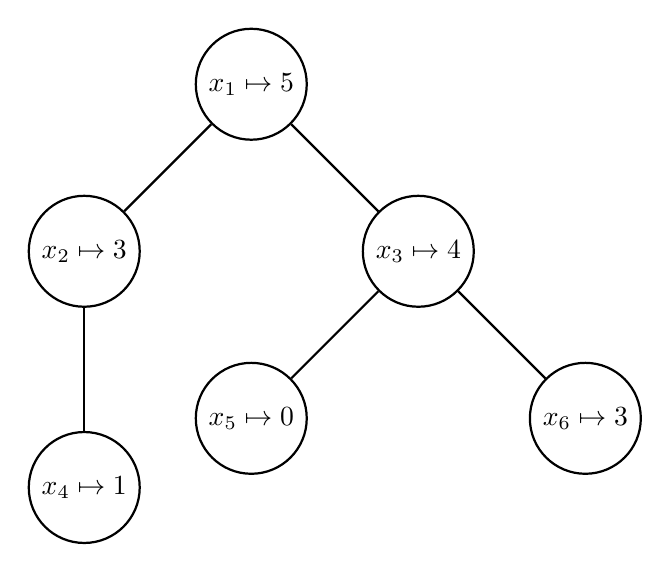
\begin{tikzpicture}[node distance={30mm}, thick, main/.style = {draw, circle}] 
\node[main] (1) {$x_1\mapsto 5$}; 
\node[main] (2) [below left of=1] {$x_2\mapsto 3$}; 
\node[main] (3) [below right of=1] {$x_3\mapsto 4$}; 
\node[main] (4) [below of=2] {$x_4\mapsto 1$}; 
\node[main] (5) [below left of=3] {$x_5\mapsto 0$}; 
\node[main] (6) [below right of=3] {$x_6\mapsto 3$}; 
\draw (1) -- (2); 
\draw (1) -- (3); 
\draw (2) -- (4); 
\draw (3) -- (5); 
\draw (3) -- (6); 
\end{tikzpicture} 

\end{center}

Then $\omega^-(x_1)=x_4$. So $\omega$ maps 
to local minimums, but not necessarily to absolute ones,
even when restricting to the same connected component. 


\end{example}


\section{Brief description of the algorithm}

With this in mind we can describe what the algorithm is. Each
iteration of the algorithm 
is separated in 6 steps.

As mentioned at the beginning of the chapter we try to progressively build a 
graph around some discrete set $X\subset M$. We start by setting
$T[0]$ to be the NNG graph of $X$.

We also set the critical points of index $0$ (that is the minimums) 
$\sigma_0^k$ to be the image under $\omega^-$
of $T[0]$.
We will need one final definition:

\begin{definition}[Bifurcating lower link]
    Let $X$ be a finite set with a Morse function $f$, and $G$ a graph on $X$.
    Given $x\in X$, we call lower link of $x$ and denote $L^-\vert_G$ to the 
    set:
    $$
        \{y\in X: \{x,y\} \text{ is and edge of } G \text{ and } f(y)\leq f(x)\}
    $$
    
    We call the bifurcating lower link of $x$ and denote $L^{-\rightsquigarrow}\vert_G$
\end{definition}


Now we described how the algorithm wokrs:
As mentioned before, if $n$ is the dimension of $M$,
we iterate $n$ times. 
From now on $k$ is the iteration count.

At the beginning of iteration $k$ we may assume 
that the following are known:

\begin{itemize}
    \item The critical points of index $k-1$.

    \item The global thickening of order $k-1$: $T[k-1]$.

    \item The set $T[k-1]$ has been sorted by increasing value of the function $f$.
\end{itemize}

On each iteration we do the following:



\begin{itemize}

    \item {\bf Step 1}
        In the first step we idenitify two important sets:
        
        \begin{itemize}
            \item {\bf Bifurcating samples}: 
                $
                B[k]
                =\{
                    x\in X: \text{
                        Vertices of } T[k-1] \text{ so that every two differents elements
                        from the lower link flow to different critical points
                    }
                \}
                $
            \item {\bf Confluence samples}: 
                $
                B[k]
                =\{
                    x\in X: \text{
                        Vertices of } T[k-1] \text{ so that every element
                        from the lower link flow to different critical points
                    }
                \}
                $

                Confluence samples usually indicate that we have reduced several flow lines
                to a single point. That is, confluence samples can be eliminated by increasing the number of samples in a neighbourhood of the confluence
                sample.

                For example in example \ref{ex1} both $x_1$ and $x_3$ are confluence samples.
        \end{itemize}


    \item {\bf Step 2}
        In this step we use the bifurcating samples to enlarge $T[k-1]$

        \begin{definition}[Anchor and Hooks]
            We call a $k$-hook any set of critical points of index $k-1$.

            Given $p\in X$ we call the anchor of $p$ the maximal hook that includes
            $\omega^-(p)$
            and
            $\omega^-(
                L^{-\rightsquigarrow}(p)
            )$
        \end{definition}


        \begin{definition}[Local thickenings]
            We define $T(A^{(k)})$ as the set of all elements from $B[k]$ having the same anchor
            and we call it the local thickening of the anchor $A^{(k)}$.       


            The lower boundary of $T(A^{(k)})$
            is defined as the elemenits of $T(A^{(k)})$ that have a lower link lying in $T[k-1]$.
        \end{definition}

        Local thickening have an associated thickness:

        \begin{definition}[Open local thickening]
        \end{definition}

    \item {\bf Step 3}
        
    \item {\bf Step 4}

    \item {\bf Step 5}

    \item {\bf Step 6}

\end{itemize}

\section{Some observations on the algorithm}

The algorithm makes some unusual (or maybe original) constructions. In this
section we explore their raison d'\^etre.

\subsection{The point of the thickenings}

Suppose we had two points in $M$, $p_i,p_j$ and $q$, 
and we have: $W(p,q_i)\cap W(q_j,p)=\{p\}$.
However, it is not possible that the stable manifold of a critical point be reduced to a
singleton.


\section{Lala}
